\section{壁の反射強度}

  実験場所である,千葉工業大学津田沼キャンパス2号館3階の廊下の壁の反射強度を計測した.実験の様子を\figref{Fig:RobotGuidance_exp1_wall}に示す.2DLiDARを壁に向けて正面に配置し,距離によって反射強度の値が変化するのを防ぐため,壁から約500 \,[mm]離れたところに固定した.また,約250秒間データを収集した.
  計測した結果を\figref{Fig:Normal distribution of reflection intensity of wall}に示す.平均値は約3600であり,分散は約546であった.

  \begin{figure}[h]
    \centering
    \begin{minipage}[c]{65mm} 
        \centering
        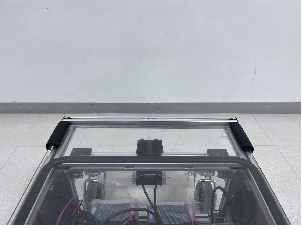
\includegraphics[height=40mm]{images/pdf/RobotGuidance_exp1_wall_from_back}
        \subcaption{View from behind}
    \end{minipage}
    \begin{minipage}[c]{65mm} 
        \centering
        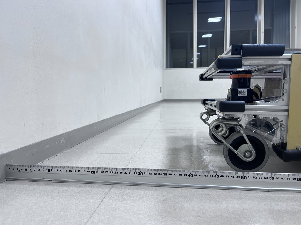
\includegraphics[height=40mm]{images/pdf/RobotGuidance_exp1_wall_from_side}
        \subcaption{View from the side}
    \end{minipage}
    \caption{Measure the reflection intensity of the wall}
    \label{Fig:RobotGuidance_exp1_wall}
  \end{figure}

  \begin{figure}[h]
    \centering
    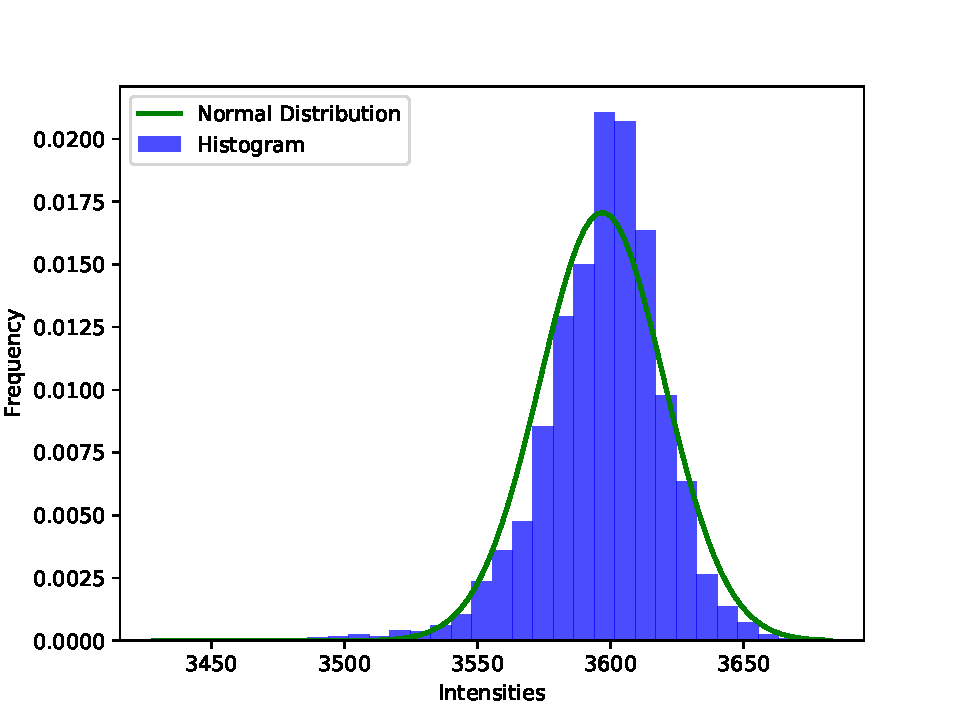
\includegraphics[keepaspectratio, scale=0.55] {images/pdf/RobotGuidance_plot_reflection_intensities_of_wall}
    \captionsetup{justification=raggedright} % キャプションを左寄せに
    \caption{Histogram of reflection intensity of wall}
    \label{Fig:Normal distribution of reflection intensity of wall}
  \end{figure}

\newpage